\chapter{Nozioni}

In questo capitolo si trattano in breve alcuni concetti ripresi spesso in questa tesi. Al fine di evitare che queste nozioni vengano date successivamente, mentre si approfondiscono altri argomenti, si è deciso di realizzare questo capitolo introduttivo che possa aiutare il lettore in una più chiara e lineare comprensione del testo. 

\section{Geometria di una faglia}
Un terremoto ha origine dall'improvviso scorrimento tra due blocchi della superficie terrestre lungo una superficie chiamata faglia.
Studiare la geometria della faglia risulta fondamentale per comprendere come è avvenuto il moto relativo tra i blocchi e per descrivere al meglio il terremoto.
Uno schema di come viene descritta una faglia è disponibile in Fig.\ref{fig:faglia}.
Tra i parametri che descrivono la faglia è possibile identificare:
\begin{itemize}
    \item \( \hat{n} \): vettore normale al piano di faglia che separa il blocco inferiore (in inglese \textit{foot wall block}) dal blocco superiore (\textit{upper hanging wall block}, non mostrato in figura)
    \item Slip (\(\vec{d}\)): vettore che descrive il moto relativo del blocco superiore rispetto a quello inferiore
    \item Traccia della faglia: retta che si ottiene intersecando il piano di faglia con la superficie terrestre (in Fig\ref{fig:faglia} coincide con la direzione \(x_1\))
    \item Strike (\(\Phi_f\)): angolo misurato sulla superficie terrestre tra il nord geografico e la traccia della faglia (\( 0^{\circ} \le \Phi_f \le 360^{\circ} \))
    \item Dip (\(\delta\)):  angolo tra la superficie terrestre e il piano di faglia (\( 0^{\circ} \le \delta \le 90^{\circ} \))
    \item Rake (o \textit{slip angle}, \(\lambda\)): angolo fra lo slip \( \vec{d} \) e la direzione della traccia della faglia (\( -180^{\circ} \le \lambda \le 180^{\circ} \))
\end{itemize}

\begin{figure}[H]
    \centering
    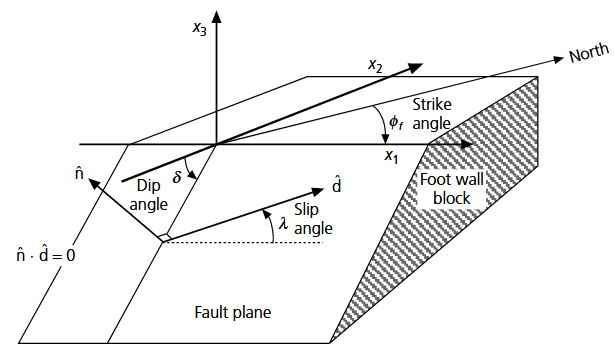
\includegraphics[width=0.85\linewidth]{graphics/faglia.png}
    \caption{Geometria di una faglia (preso da \citet{introduction_to_seismology}).}
    \label{fig:faglia}
\end{figure}

TODO: fare citazione di questa sezione, ho usato solo \citep{introduction_to_seismology} e note di fluidi, inoltre nella figura in realta ho citato una figura che è però stata citata a sua volta, cito originale?

\subsection{Classificazione delle faglie}
A seconda di come avviene lo scorrimento tra i due blocchi lungo il piano di faglia possiamo classificare diversi tipi di faglie, raffigurati in Fig.\ref{fig:tipi_faglia}, descritti in base a specifici valori del rake \(\lambda\):

\begin{itemize}
    \item faglia trascorrente (\textit{strike-slip fault}): si realizza quando i due blocchi scorrono orizzontalmente l'uno rispetto all'altro. Se \( \lambda=0^{\circ} \) il movimento si dice \textit{left lateral}, se \( \lambda=180^{\circ} \) si dice \textit{right lateral}
    \item faglia normale (\textit{normal fault}): quando si ha lo scivolamento del blocco superiore rispetto a quello inferiore, se \( \lambda=270^{\circ} \)  
    \item faglia inversa o di sovrascorrimento (\textit{reverse/thrust fault}): quando si ha la risalita del blocco superiore rispetto a quello inferiore, se \( \lambda=90^{\circ} \)
\end{itemize}

Le faglie normali e inverse sono dette anche \textit{faglie dip-slip}, in quanto il movimento relativo tra i due blocchi avviene nella direzione del dip della faglia.

\begin{figure}[H]
    \centering
    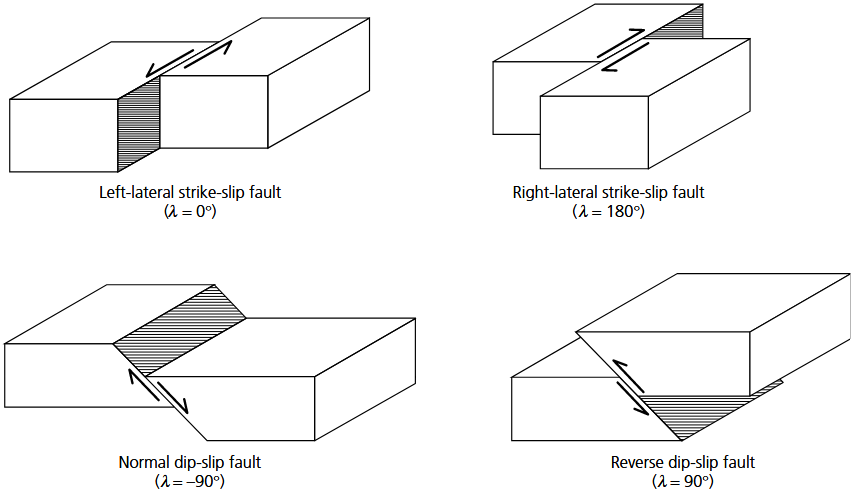
\includegraphics[width=0.85\linewidth]{graphics/tipi_faglia.png}
    \caption{}
    \label{fig:tipi_faglia}
\end{figure}


\section{Cenni di teoria della fagliazione}